\chapter{Numerische Ergebnisse}

In diesem Kapitel werden wir mit unserer persönlichen Implementierung das \Quote{Hadeler Problem}

\begin{gather*}
    T(z) = (e^z - 1) B_1 + z^2 B_2 - B_0 \\
    B_0 = b_0 I_n,
    \quad
    B_1 = (b_{j k}^{(1)}),
    \quad
    B_2 = (b_{j k}^{(2)}) \\
    b_{j k}^{(1)} = (n + 1 - \max(j, k)) j k,
    \quad
    b_{j k}^{(2)} = n \delta_{j k} + 1 / (j + k),
    \quad
    j, k = 1, \dots, n,
\end{gather*}

aus \cite{saad2020rational} lösen, und die theoretischen Ergebnisse veranschaulichen. \\
Wir legen die Parameter mit $n = 200, b_0 = 100$ fest und wählen
unsere Kurve als Kreis mit Mittelpunkt $z = -30$ und Radius $R = 11.5$.
Als Toleranz zur Bestimmung der \Quote{korrekten} Singulärwerte wählen wir $tol = 10^{-5}$. \\
Im ersten Testlauf plotten wir die berechneten Eigenwerte im Vergleich zu
den zusätzlich aussortierten Werten. Zur besseren Veranschaulichung haben wir
die Quadraturpunkte über die wir summieren auch miteingezeichnet.
Wie man in Abbildung \ref{fig:plot1} sieht befinden sich die von unserem Algorithmus als \Quote{korrekt}
identifizierten Eigenwerte alle innerhalb unserer Konturintegralkurve, während
die zusätzlichen Werte außerhalb liegen.

In Abbildung \ref{fig:plot2} sehen wir den Vergleich der Größenordnungen der
eigentlichen Singulärwerte mit den zusätzlichen Singulärwerten. Nachdem in diesem
Fall ein deutlicher Abfall zu erkennen ist, ist es nicht schwer die zusätzlichen
Werte auszusortieren.

Eine Heuristik zur Überprüfung der Qualität unserer approximierten Eigenwerte
ist es, die Konditionszahl der jeweiligen Matrix $A(\lambda)$ zu betrachten.
Da wir gegen eine singuläre Matrix konvergieren sollten, würden wir erwarten,
dass die Konditionszahl gegen unendlich geht. In der Tat ist das Fall und
man erkennt in Abbildung \ref{fig:plot3} sogar einen deutlichen Unterschied
zwischen den echten und zusätzlichen Eigenwerten.

Schlussendlich wollen wir noch Situationen aufzeigen, an denen der Algorithmus
scheitert. Die erste Möglichkeit dafür besteht darin, dass die Quadratur zu
ungenau ist, und somit die \Quote{korrekten} Singulärwerte nicht mehr von den
zusätzlichen Werten zu unterscheiden sind. In Abbildung \ref{fig:plot4} sieht
man, wie sich die approximierten Singulärwerte bei unterschiedlicher Anzahl
von Quadraturknoten verhalten. Ab 20 Quadraturknoten aufwärts ist bereits
ein Sprung zwischen den echten und zusätzlichen Werten zu erkennen, der sich
bei steigender Anzahl noch verdeutlicht.

Das zweite Hauptproblem, was auftreten kann ist, wenn die Zufallsmatrix zu klein
gewählt wird. Sollte die Zufallsmatrix weniger Spalten haben als wir
Eigenwerte innerhalb unserer Kurve erwarten, könnte ja man noch hoffen,
zumindest einen Teil der Eigenwerte korrekt approximieren zu können.
Wie man in Abbildung \ref{fig:plot5} sieht, können wir in der Regel nicht
einmal das erwarten.

\begin{figure}
  \caption{Approximierte Eigenwerte vs. zusätzliche Werte}
  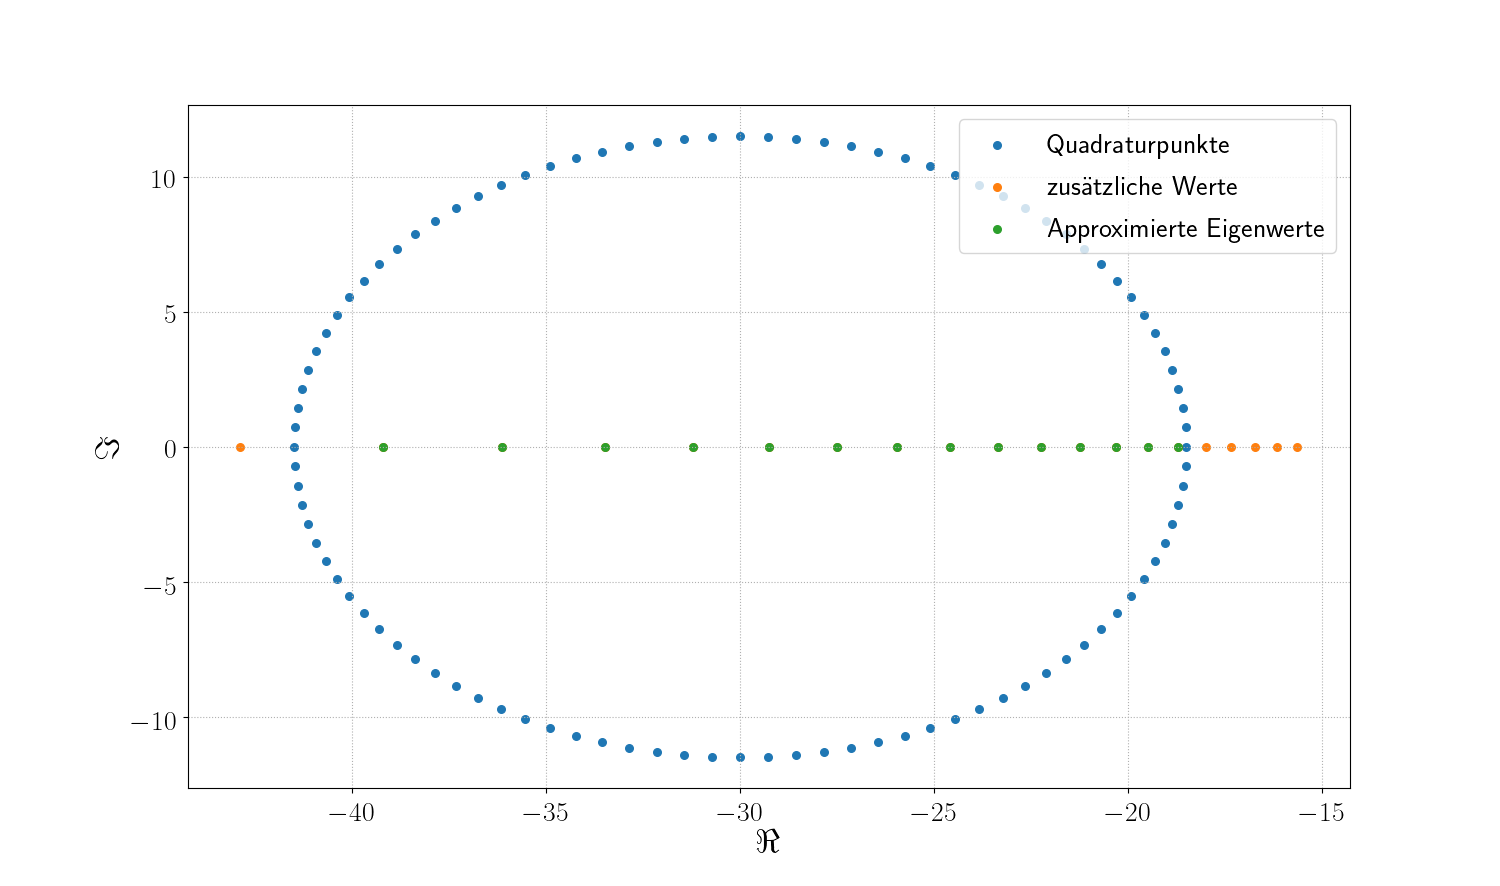
\includegraphics[width=\linewidth]{Plots/eigenwerte_complex_plot.png}
  \label{fig:plot1}
\end{figure}

\begin{figure}
  \caption{Konditionszahlen von $A(\lambda_n)$}
  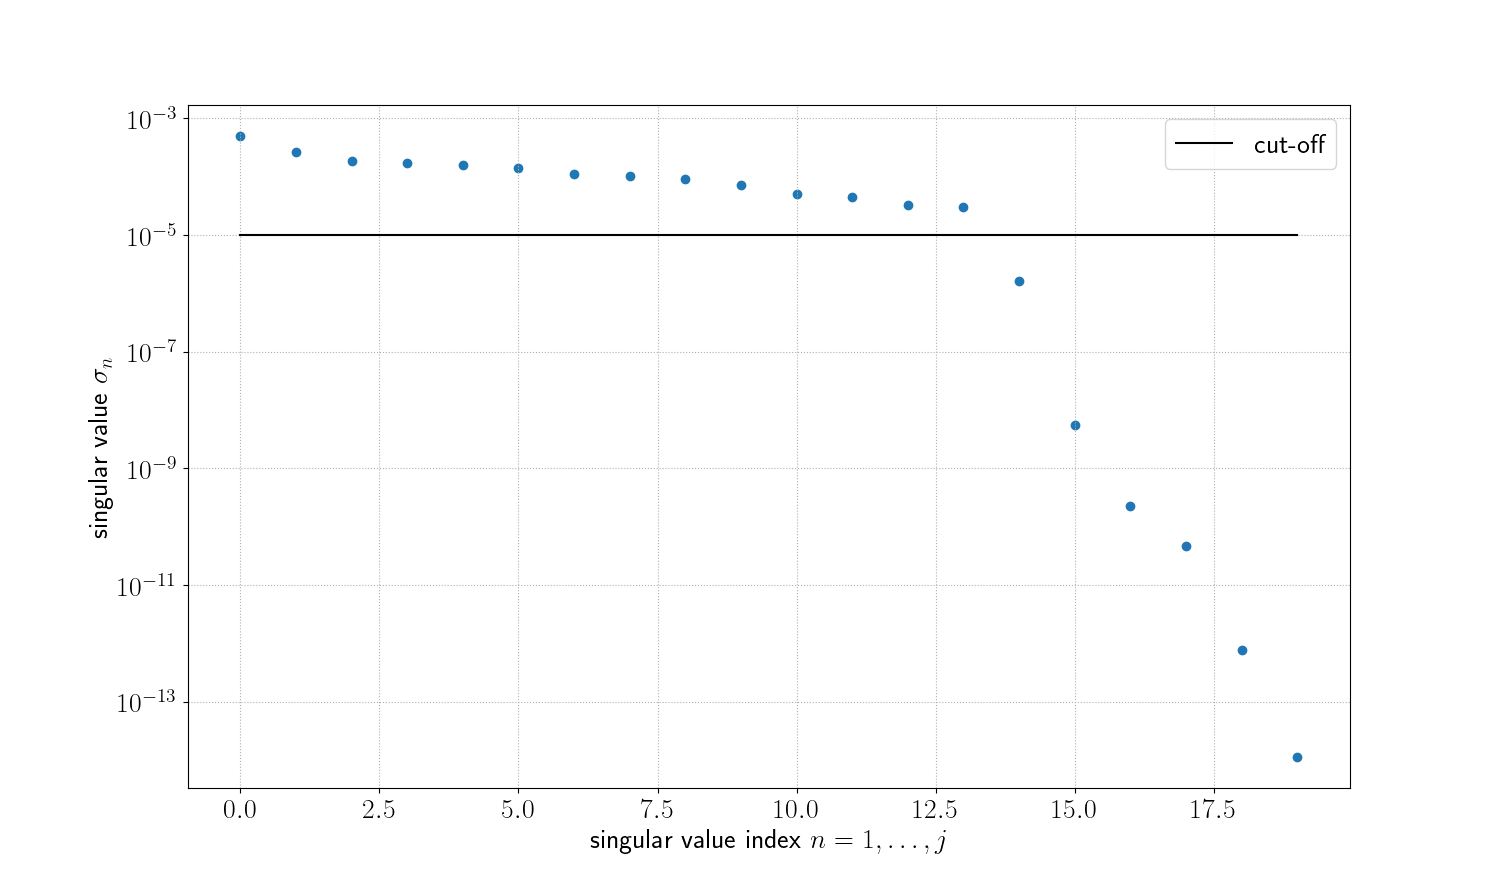
\includegraphics[width=\linewidth]{Plots/singulaerwerte_plot.png}
  \label{fig:plot2}
\end{figure}

\begin{figure}
  \caption{Echte vs. zusätzliche Singulärwerte}
  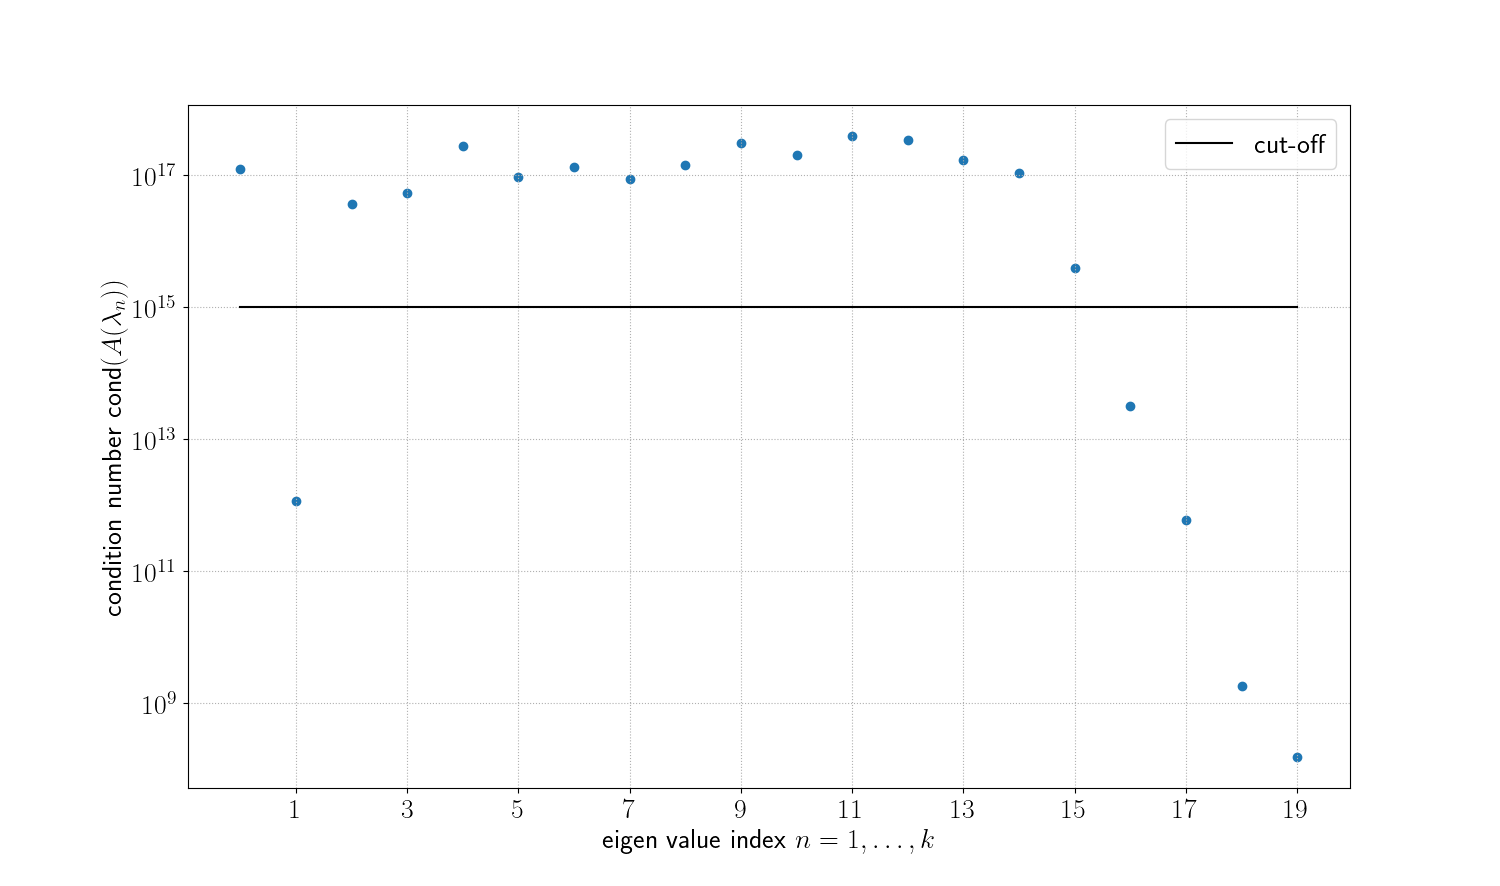
\includegraphics[width=\linewidth]{Plots/conditionnumber.png}
  \label{fig:plot3}
\end{figure}

\begin{figure}
  \caption{Singulärwerte in Abhängigkeit von der Anzahl der Quadraturknoten}
  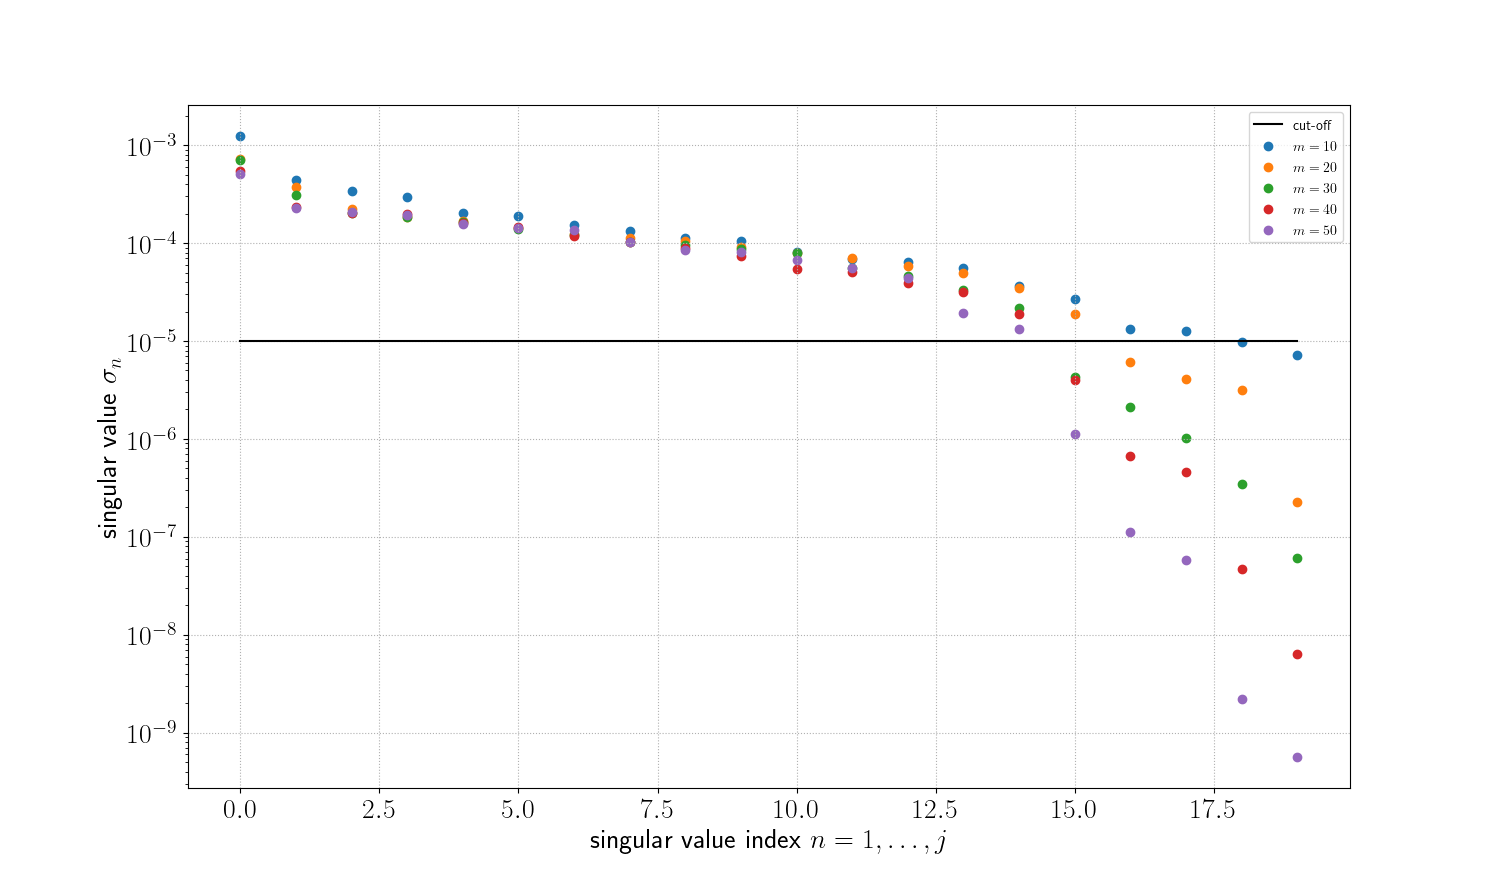
\includegraphics[width=\linewidth]{Plots/singulaerwerte_quadraturknoten.png}
  \label{fig:plot4}
\end{figure}

\begin{figure}
  \caption{Zu kleine Zufallsmatrix}
  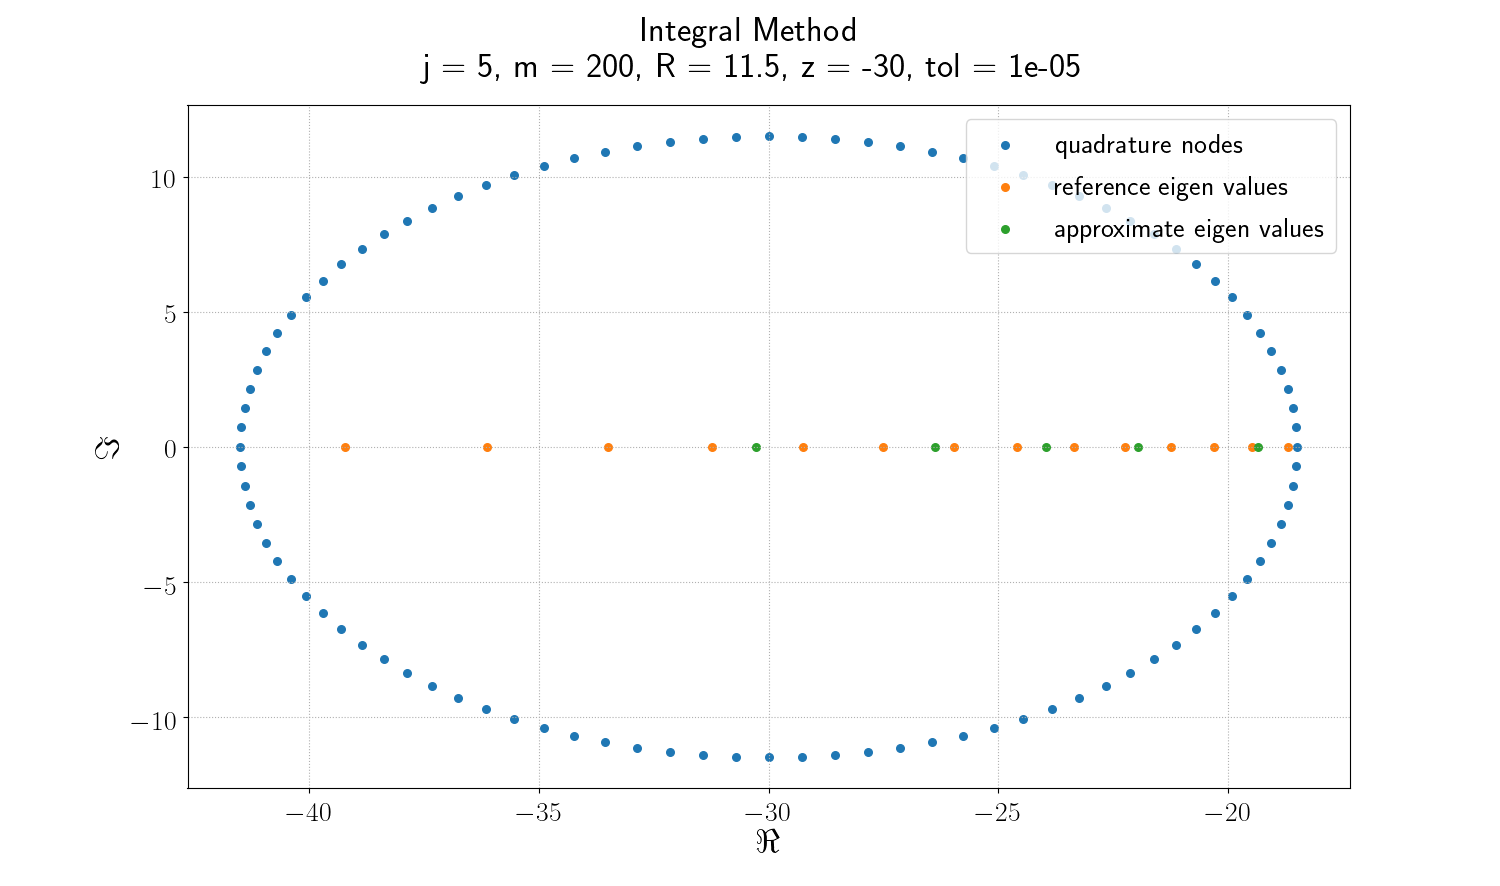
\includegraphics[width=\linewidth]{Plots/zufallsmatrix_zu_klein.png}
  \label{fig:plot5}
\end{figure}
